\RequirePackage[OT1]{fontenc} 
\documentclass[journal]{IEEEtran}

% *** CITATION PACKAGES ***
\usepackage[style=ieee]{biblatex} 
\bibliography{example_bib.bib}    %your file created using JabRef

% *** MATH PACKAGES ***
\usepackage{amsmath}

% Table Packages
\usepackage{booktabs}
\usepackage{tabularx}

% *** PDF, URL AND HYPERLINK PACKAGES ***
\usepackage{url}
% correct bad hyphenation here
\hyphenation{op-tical net-works semi-conduc-tor}
\usepackage{graphicx}  %needed to include png, eps figures
\graphicspath{{./images/}}
\usepackage{float}  % used to fix location of images i.e.\begin{figure}[H]

\begin{document}

% paper title
\newcommand{\LabNumber}{\#4}
\newcommand{\LabTitle}{Microstrip Transmission Lines}

\title{RF Lab Module \LabNumber\ --- \LabTitle}
%\\ \small{Title of the session (you can be creative highlighting your findings)}}

% author names 
\author{Stephen Campbell
    % Student 2 First Name Last Name 
}% <-this % stops a space

% The report headers
\markboth{EE/CE 4202 Electrical and Computer Engineering Laboratory in Circuits. Lab \LabNumber, \today}%do not delete next lines
{Shell \MakeLowercase{\textit{et al.}}: Bare Demo of IEEEtran.cls for IEEE Journals}

% make the title area
\maketitle

% As a general rule, do not put math, special symbols or citations
% in the abstract or keywords.
\begin{abstract}
    Microstrip transmission lines are of utmost importance to RF engineers around
    the globe due to their ease of design and fabrication. In this lab, microstrip
    transmission lines are designed, fabricated, measured, and analyzed in order to
    gain insight and build trust in the theoretical model of the microstrip
    transmission line.
\end{abstract}

\section{Introduction}

\IEEEPARstart{A}{n}
An online calculator was used to design the microstrip transmission line.
Using the width provided by this calculator the microstrip was able to be
fabricated. Several fabrication materials utilized in this lab include a
dielectric board laminated with a copper sheet and copper tape. With the
microstrip transmission line constructed, its S-parameters were measured using
the Agilent VNA utilized in previous labs. Using this data, the characteristic
impedance was determined and compared to the desired value.

\section{Analysis}

\textbf{If your line is 4” (or write your length) long, how long is that electrically at 5 GHz?}
\begin{align*}
    L                  & =4\text{in}                                                  \\
    L                  & =4\text{in}\frac{2.54\cdot 10^{-2}\text{m}}{1\text{in}}      \\
    L                  & =1.016\times 10^{-1}\text{m}                                 \\
    f                  & =5\times 10^{9}                                              \\
                       & \text{Free Space}                                            \\
    c                  & =\lambda f                                                   \\
    \lambda            & =\frac{c}{f}                                                 \\
    \lambda            & =\frac{3\times 10^{8}}{5\times 10^{9}}                       \\
    \lambda            & =6\times 10^{-2}\text{m}                                     \\
    \frac{L}{\lambda } & =\frac{1.016\times 10^{-1}\text{m}}{6\times 10^{-2}\text{m}} \\
    \frac{L}{\lambda } & =1.6833                                                      \\
    L                  & =1.6833\lambda
\end{align*}

\textbf{How did you check for DC connectivity? What things did you connect together to ensure proper connections?}

To check for DC connectivity a multimeter was used. The multimeter was placed in
the ohmmeter mode and a single connection was checked per board. The signal
layer i.e.\ the copper tape was connected to one lead and the bottom ground plane
layer was connected to the other lead. The ohmmeter was read and confirmed not
to be 0 ohms or shorted.  If it the connection was shorted then our microstrip
transmission lines would not behave as expected. Thus to ensure it worked as
expected, the ground and signal layers were confirmed not to be connected.

\textbf{What are the pros and cons of using microstrip transmission lines?}
There are many advantages and disadvantages to manufacturing transmission lines with microstrip.
Many of the advantages of microstrip are:
\begin{itemize}
    \item Ease of manufacture
    \item Ease of design
    \item Wide availability
    \item Overall Cost
\end{itemize}
Some of the disadvantages microstrip are:
\begin{itemize}
    \item Susceptibility to electromagnetic interference
    \item Can become significantly lossy at highs frequencies
\end{itemize}


\section{Discussion and Summary}

Overall, considering the fabrication tolerances utilized in this procedure the
measurements seen in this lab accurately correspond to the theoretical model
discussed in lecture. Some errors may include:
\begin{itemize}
    \item Accuracy and consistency of the width of the cut microstrip line
    \item Poor SMA-board connections due to poor soldering
\end{itemize}

\appendices
\section{Pre-Lab}


\begin{figure}[hp]
    \centering
    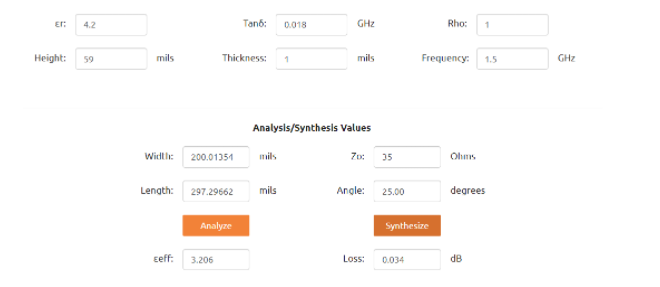
\includegraphics[width=0.3\textwidth]{design_35.png}
    \caption{35 Ohm Microstrip Transmission Line Prelab Design Calculation}
\end{figure}

\begin{align*}
    Z_{0} =35 & \rightarrow w=200.01354\text{mils}                                                                                   \\
    w         & =200.01354\text{mils}\frac{1\text{in}}{1000\text{mil}}\frac{2.54\text{cm}}{1\text{in}}\frac{10\text{mm}}{1\text{cm}} \\
              & =5.08034\text{mm}
\end{align*}


\begin{figure}[hp]
    \centering
    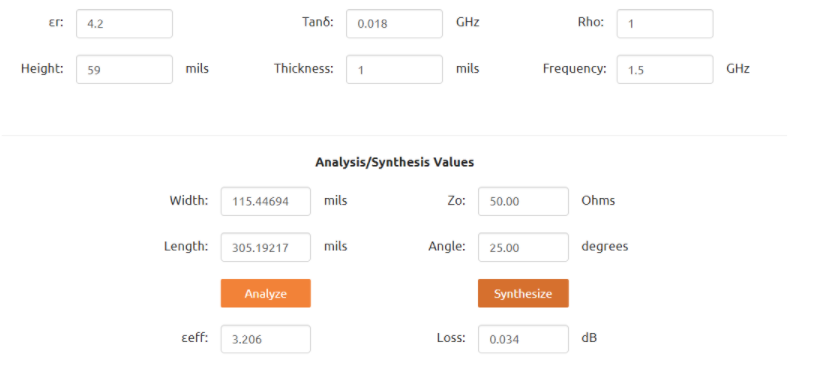
\includegraphics[width=0.3\textwidth]{design_50.png}
    \caption{35 Ohm Microstrip Transmission Line Prelab Design Calculation}
\end{figure}

\begin{align*}
    Z_{0} =50 & \rightarrow w=115.446\text{mils}                                                                                   \\
    w         & =115.446\text{mils}\frac{1\text{in}}{1000\text{mil}}\frac{2.54\text{cm}}{1\text{in}}\frac{10\text{mm}}{1\text{cm}} \\
              & =2.93233\text{mm}
\end{align*}


\section{Extra Photos}
\begin{figure}
    \centering
    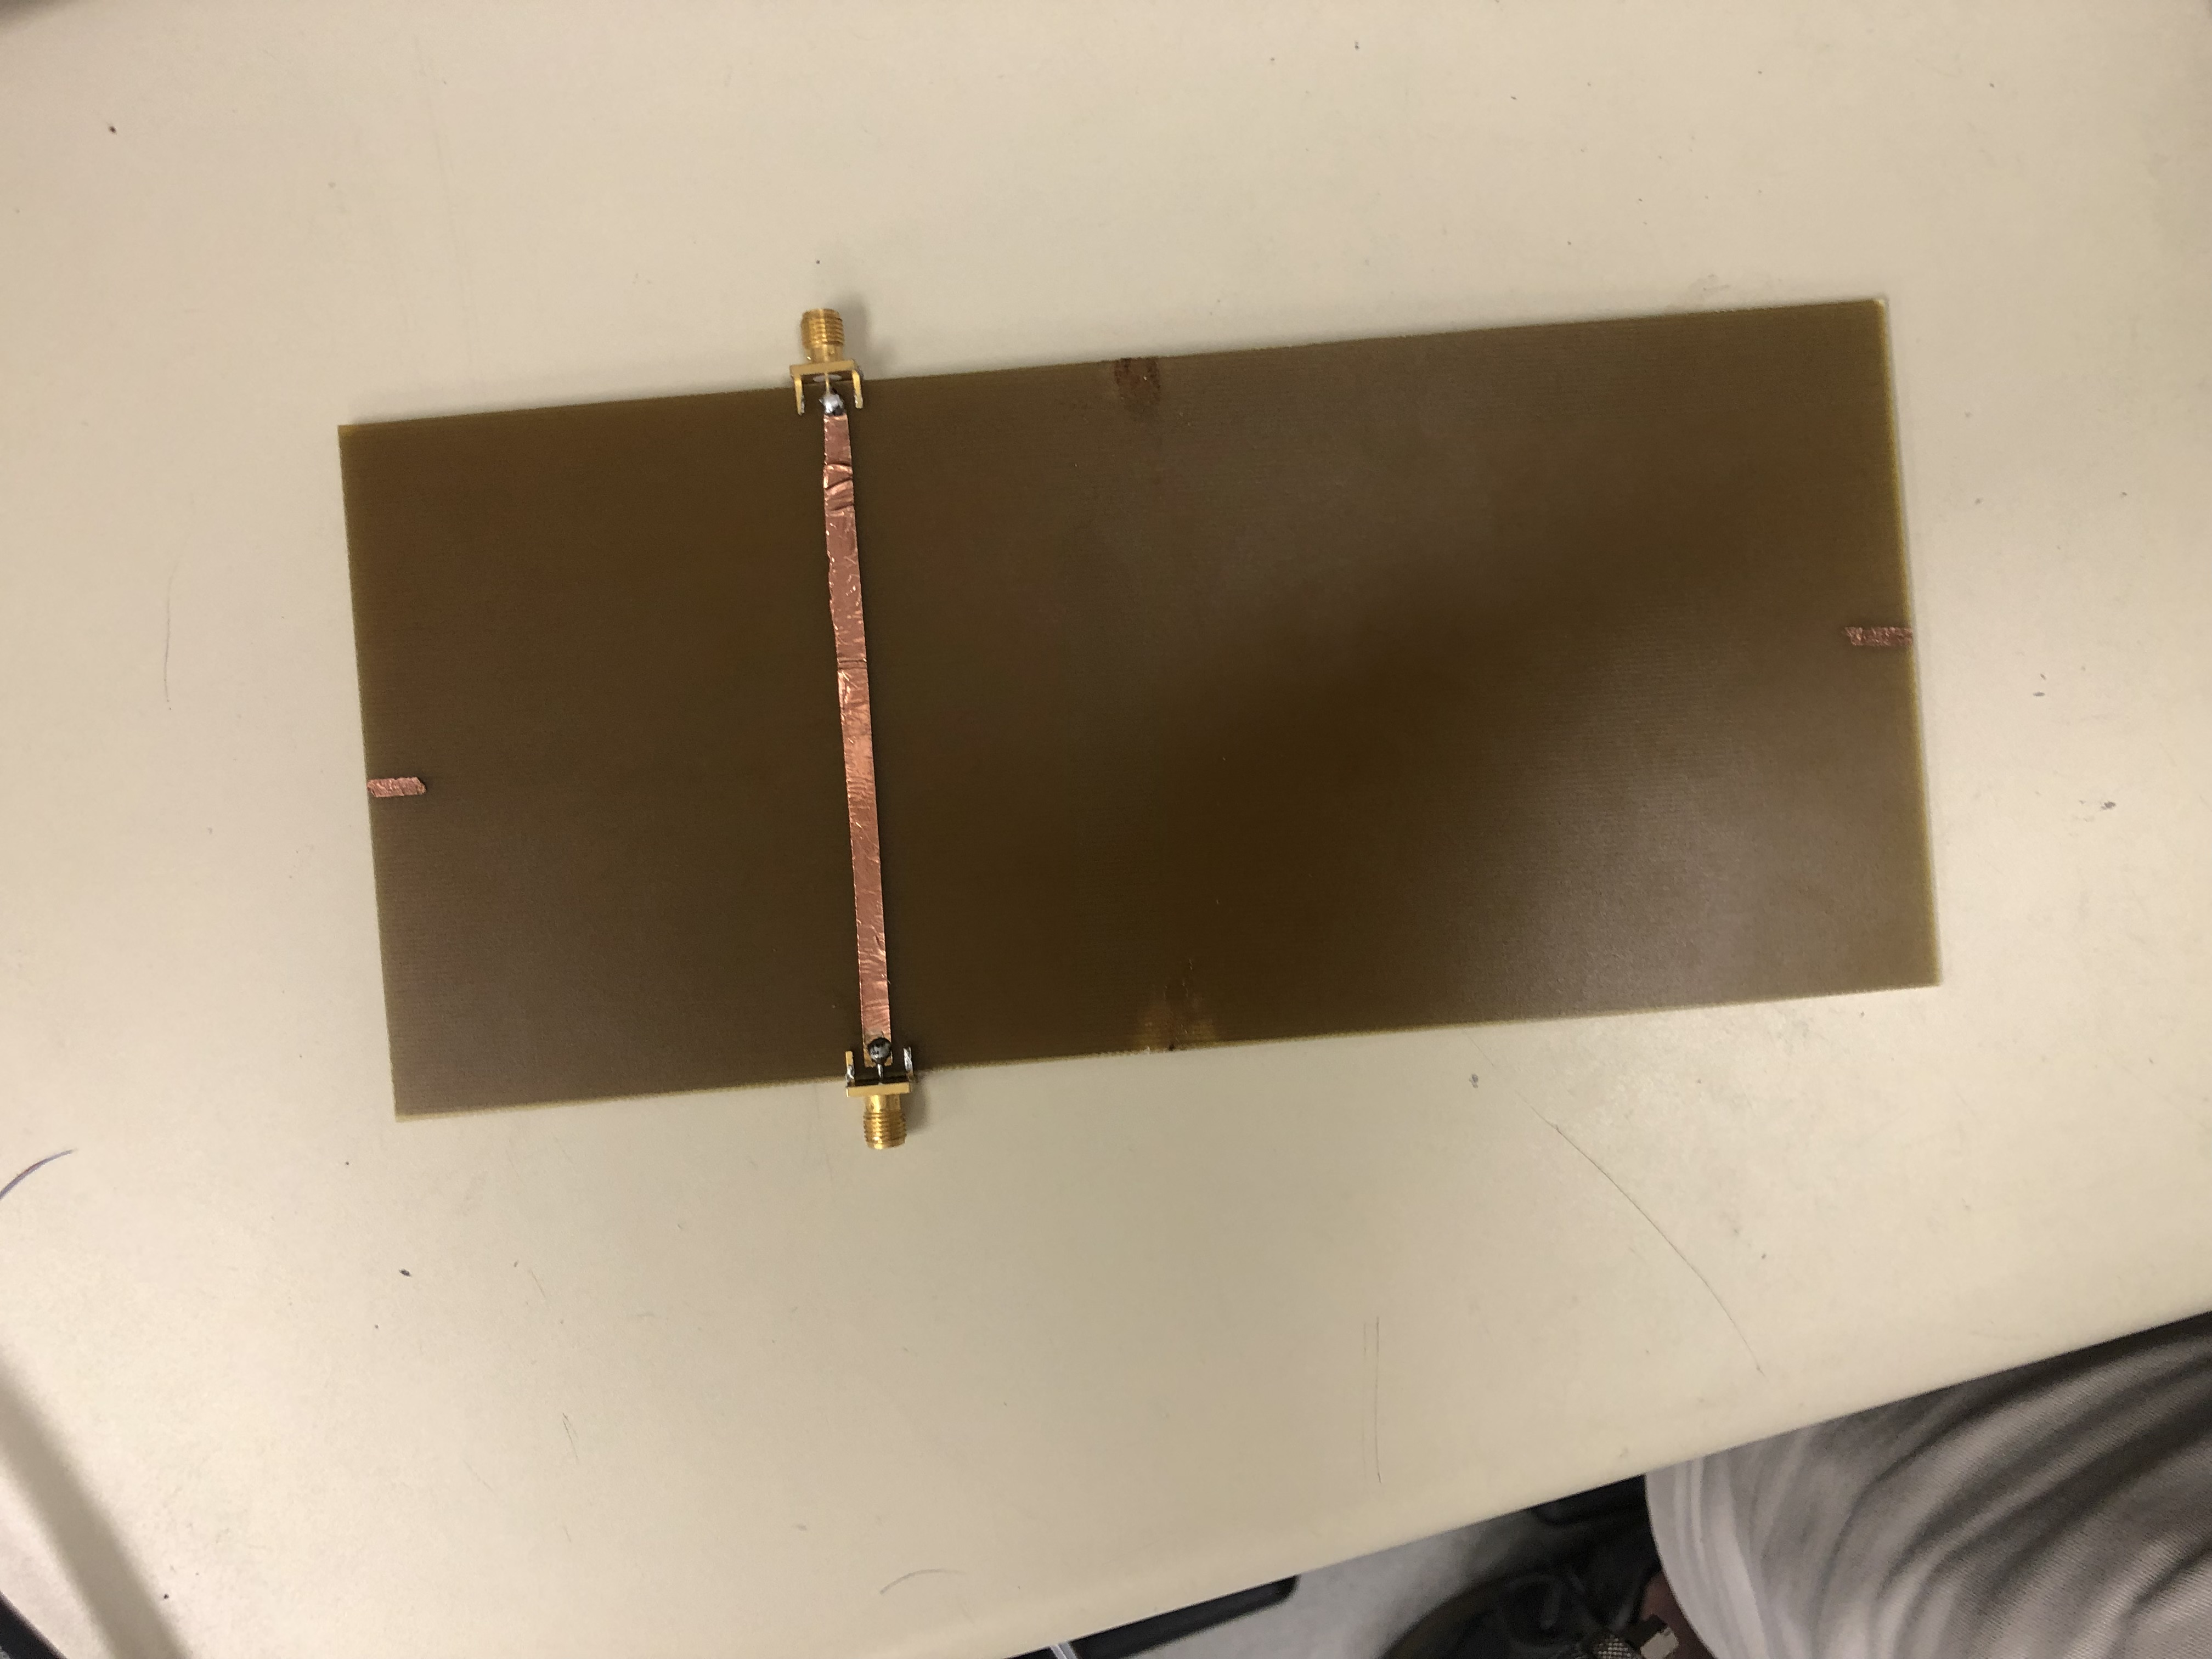
\includegraphics[width=0.3\textwidth]{microstrip_35.jpg}
    \caption{35 Ohm Microstrip Transmission Line}
\end{figure}

\begin{figure}
    \centering
    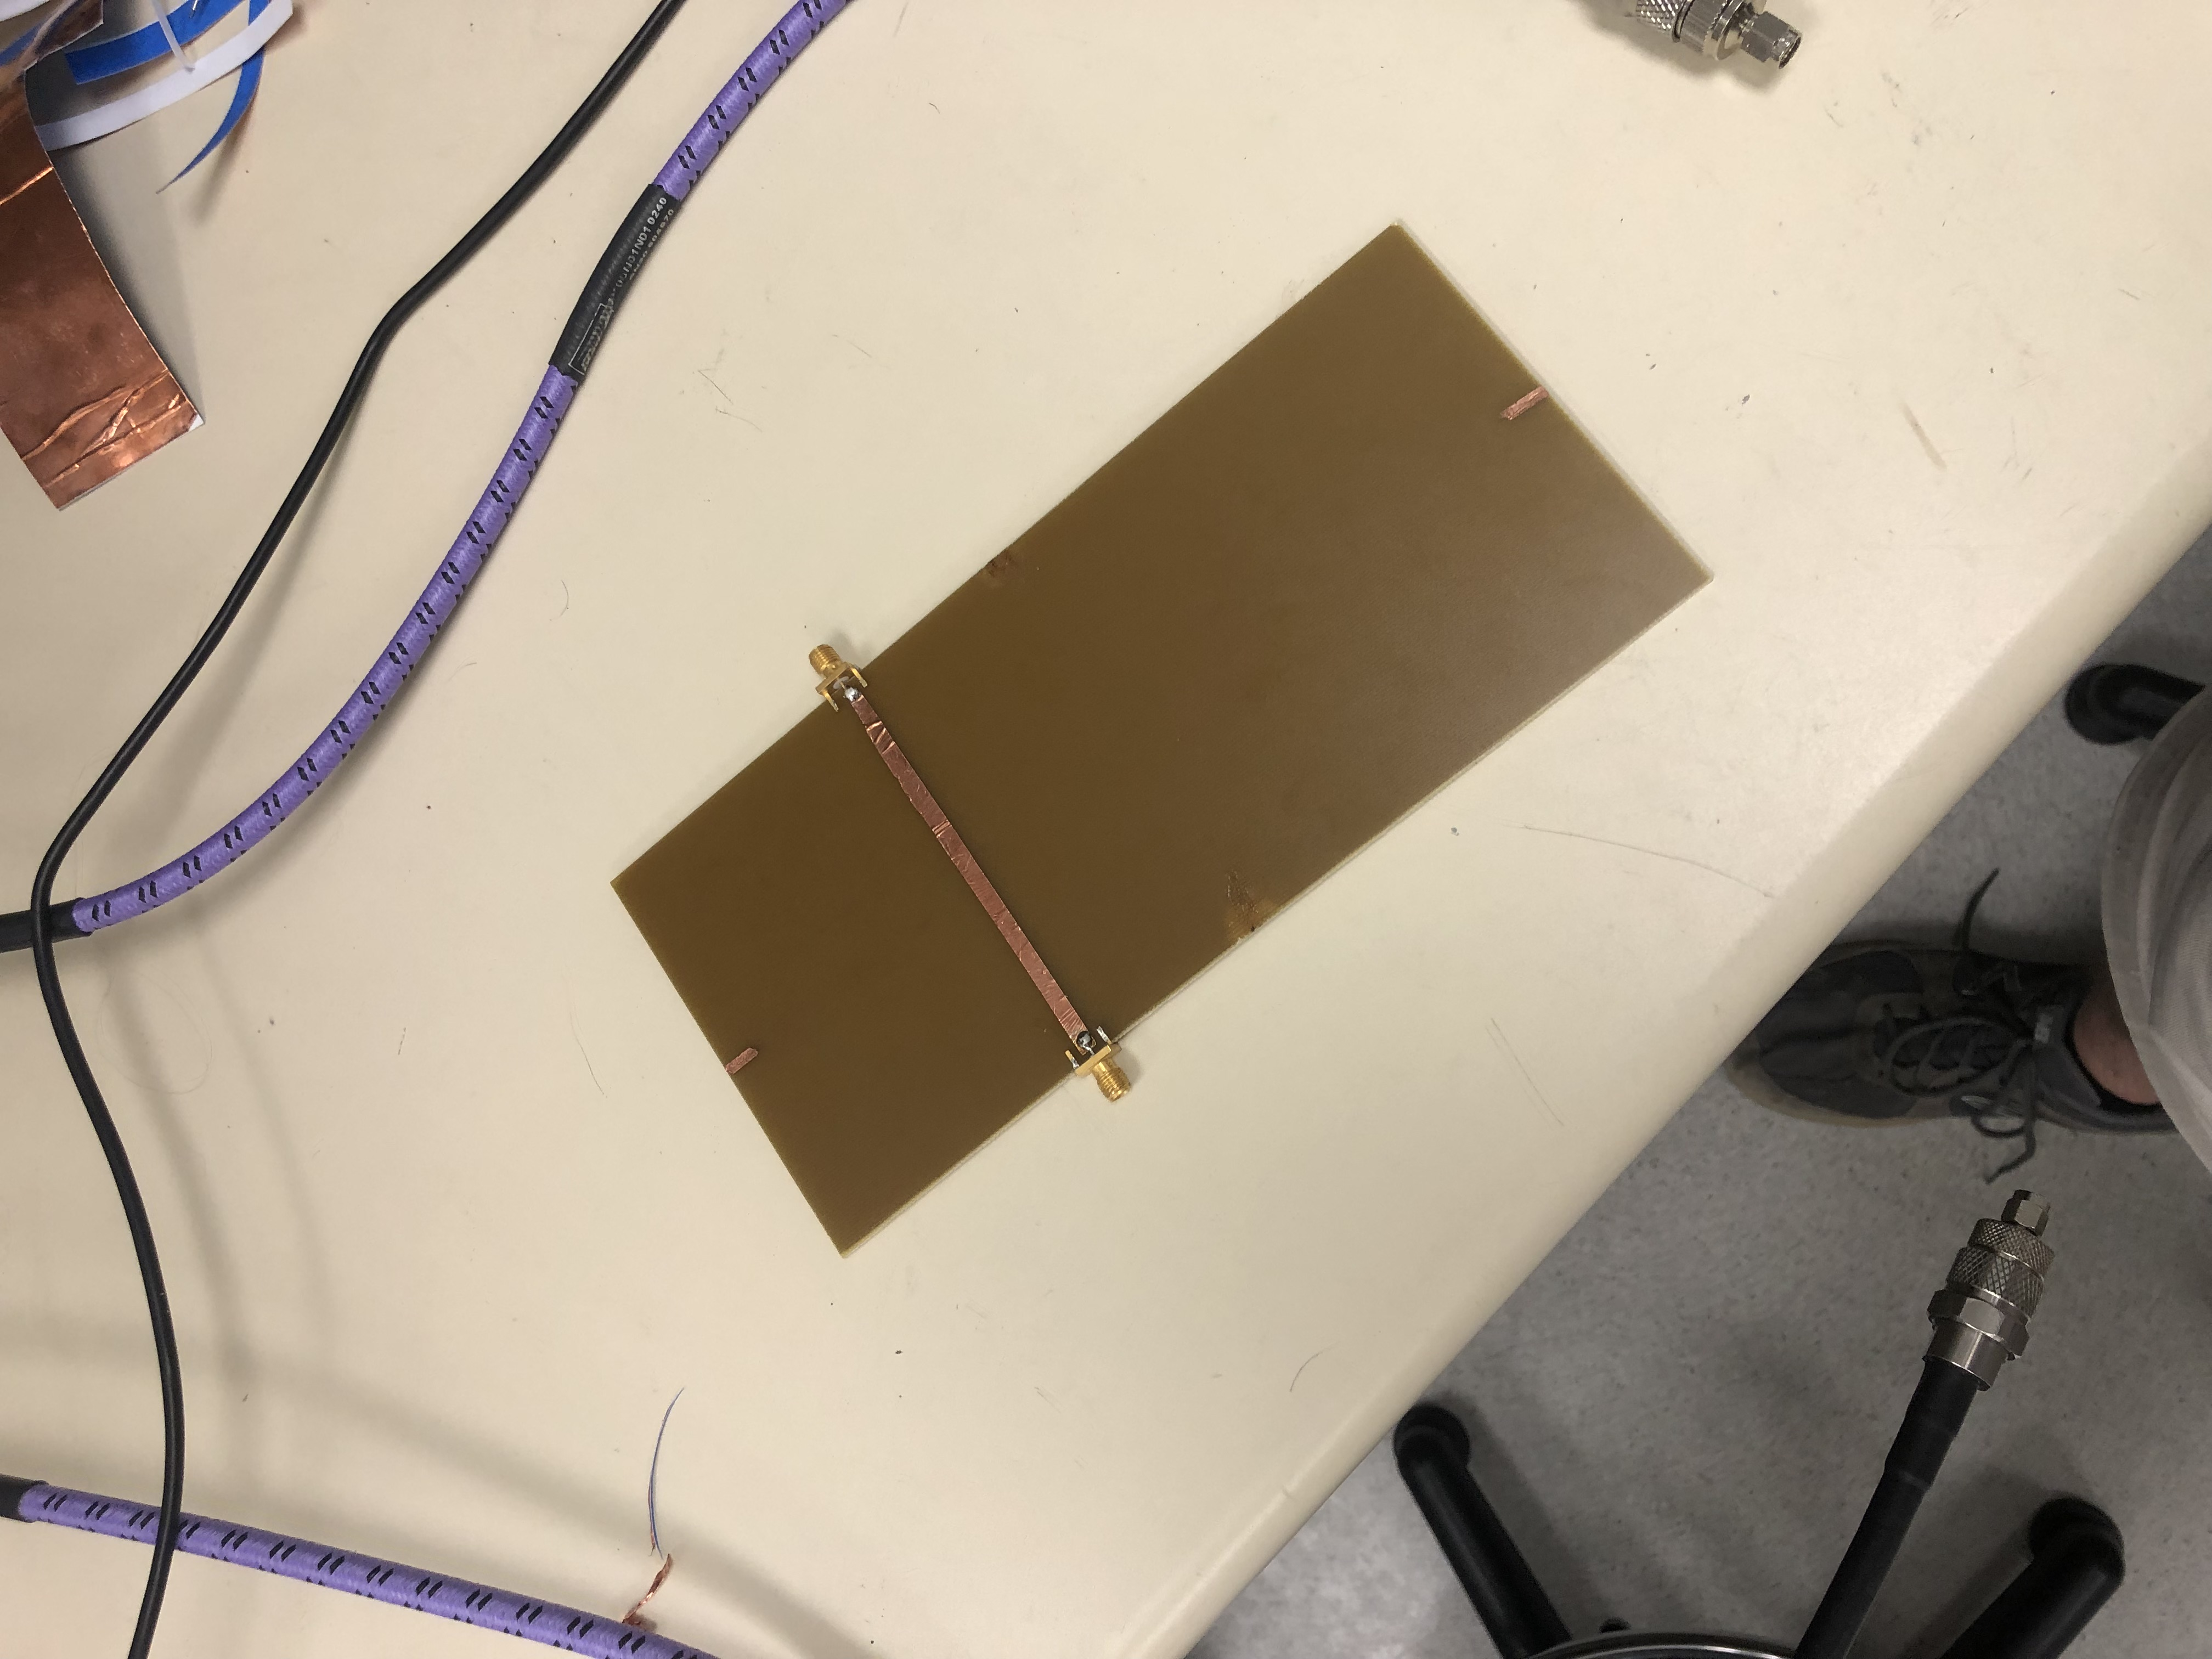
\includegraphics[width=0.3\textwidth]{microstrip_50.jpg}
    \caption{50 Ohm Microstrip Transmission Line}
\end{figure}

\end{document}